\section{Endbewertung}
\autorbeginn{Marcel}
\label{sec:ui-endbewertung}

Zur Auswertung gelangt der Spieler über einen Button auf der Spielübersicht. In der Auswertung, kann der Spieler Informationen der vergangenen Spielrunden sowie die Gesamtauswertung nach Ablauf der 10 Spielrunden einsehen.
 
Rundenweise werden die Finanzen des Unternehmens festgehalten. Dazu wird das Bankguthaben am Anfang der Runde in einer Tabelle dargestellt. Die Tabelle enthält ebenso die in der Spielrunde erhaltenen Einnahmen sowie getätigten Ausgaben. Aus diesen Informationen ergibt sich das Bankguthaben am Ende der Runde. Denkbar wäre hier bei einer Realisierung der Benutzeroberfläche, dass der Spieler zusätzlich ein Liniendiagramm, das das Bankguthaben und die Einnahmen und Ausgaben der Spielrunde enthält, angezeigt bekommt. So kann die Finanzsituation der jeweiligen Runde besser optisch dargestellt werden. Nach jeder Spielrunde wird ebenso der Star der vergangenen Runde festgehalten. Dieser wird anhand eines Bildes zentral dargestellt. (\ref{img:ui-auswertung})

\begin{figure}[h]
  \centering
  \fbox{
    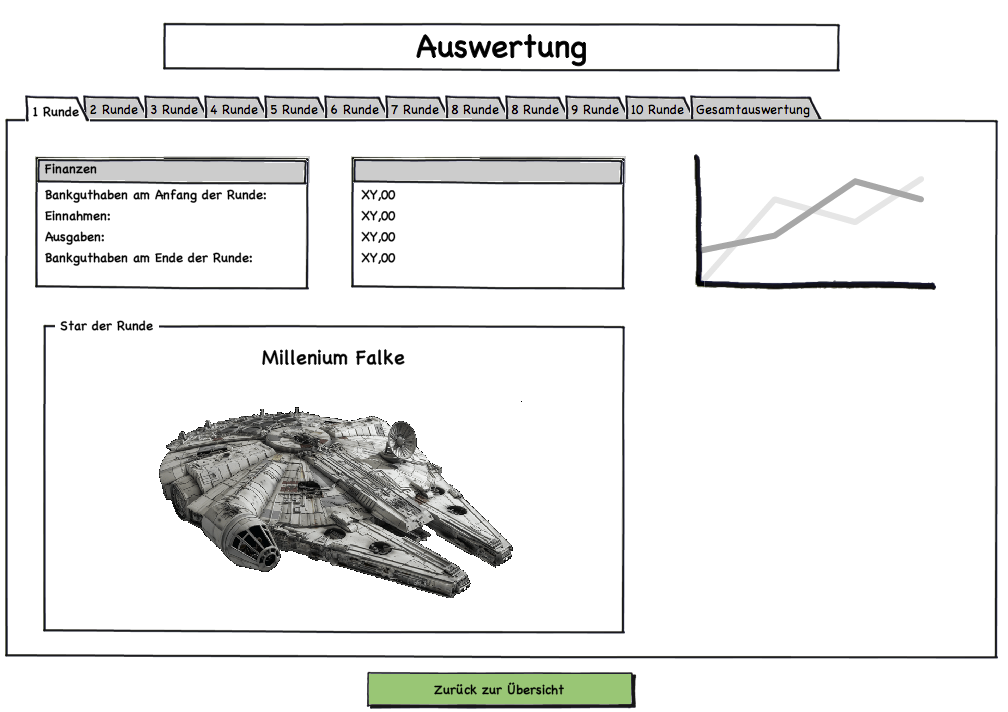
\includegraphics[width=0.9\textwidth]{40_UI/80_Endbewertung/Auswertung.png}
  }
  \caption{Auswertung pro Runde}
  \label{img:ui-auswertung}
\end{figure}
 
Die Gesamtauswertung wird nach den zehn Spielrunden ausgegeben. Sie besteht aus einer Tabelle mit den drei Spalten Rang, Unternehmen und Punktzahl.  Der Rang ist absteigend sortiert. Dies bedeutet, dass das Unternehmen auf Rang eins das Unternehmensplanspiel gewonnen hat. Die zweite Spalte enthält den Unternehmensnamen. In der letzten Spalte wird letztendlich die Punktzahl angezeigt, die der Spieler über die 10 Spielrunden erreicht hat. Damit die Berechnung der Punktzahl nachvollziehbar ist, enthält der Bildschirm zur Gesamtauswertung den Button „Berechnung der Punktzahl“. Über diesen Button gelangt der Spieler zu einem PopUp. In diesem PopUp wird dem Spieler ausführlich erläutert, aus welchen Faktoren sich die erreichte Punktzahl zusammensetzt. (\ref{img:ui-gesamtauswertung})

\begin{figure}[h]
  \centering
  \fbox{
    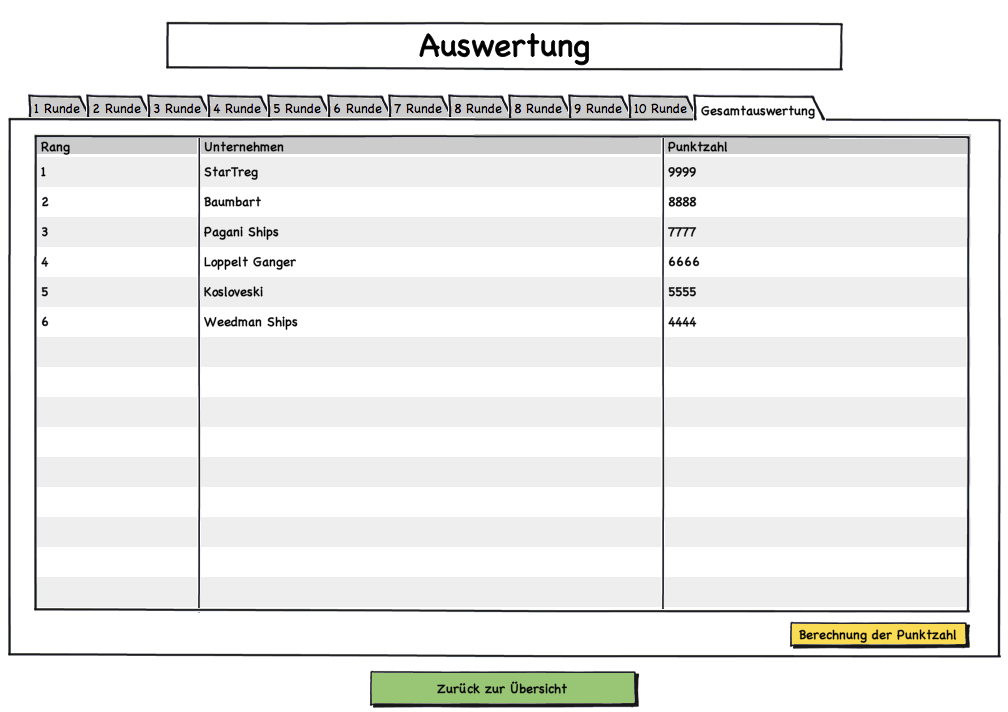
\includegraphics[width=0.9\textwidth]{40_UI/80_Endbewertung/Gesamtauswertung.png}
  }
  \caption{Auswertung pro Runde}
  \label{img:ui-gesamtauswertung}
\end{figure}
 
Die Gesamtauswertung ist der letzte erscheinende Bildschirm in dem Unternehmensplanspiel StarGreg.  Der Spieler hat zwar noch die Möglichkeit alle anderen Bildschirme einzusehen, kann aber keine Aktionen mehr ausführen. Das Spiel wird dann durch ein Schließen des Fensters beendet. 



\autorende{}